\section{dg::Window Class Reference}
\label{classdg_1_1Window}\index{dg::Window@{dg::Window}}
{\tt \#include $<$Window.h$>$}

Inheritance diagram for dg::Window:\begin{figure}[H]
\begin{center}
\leavevmode
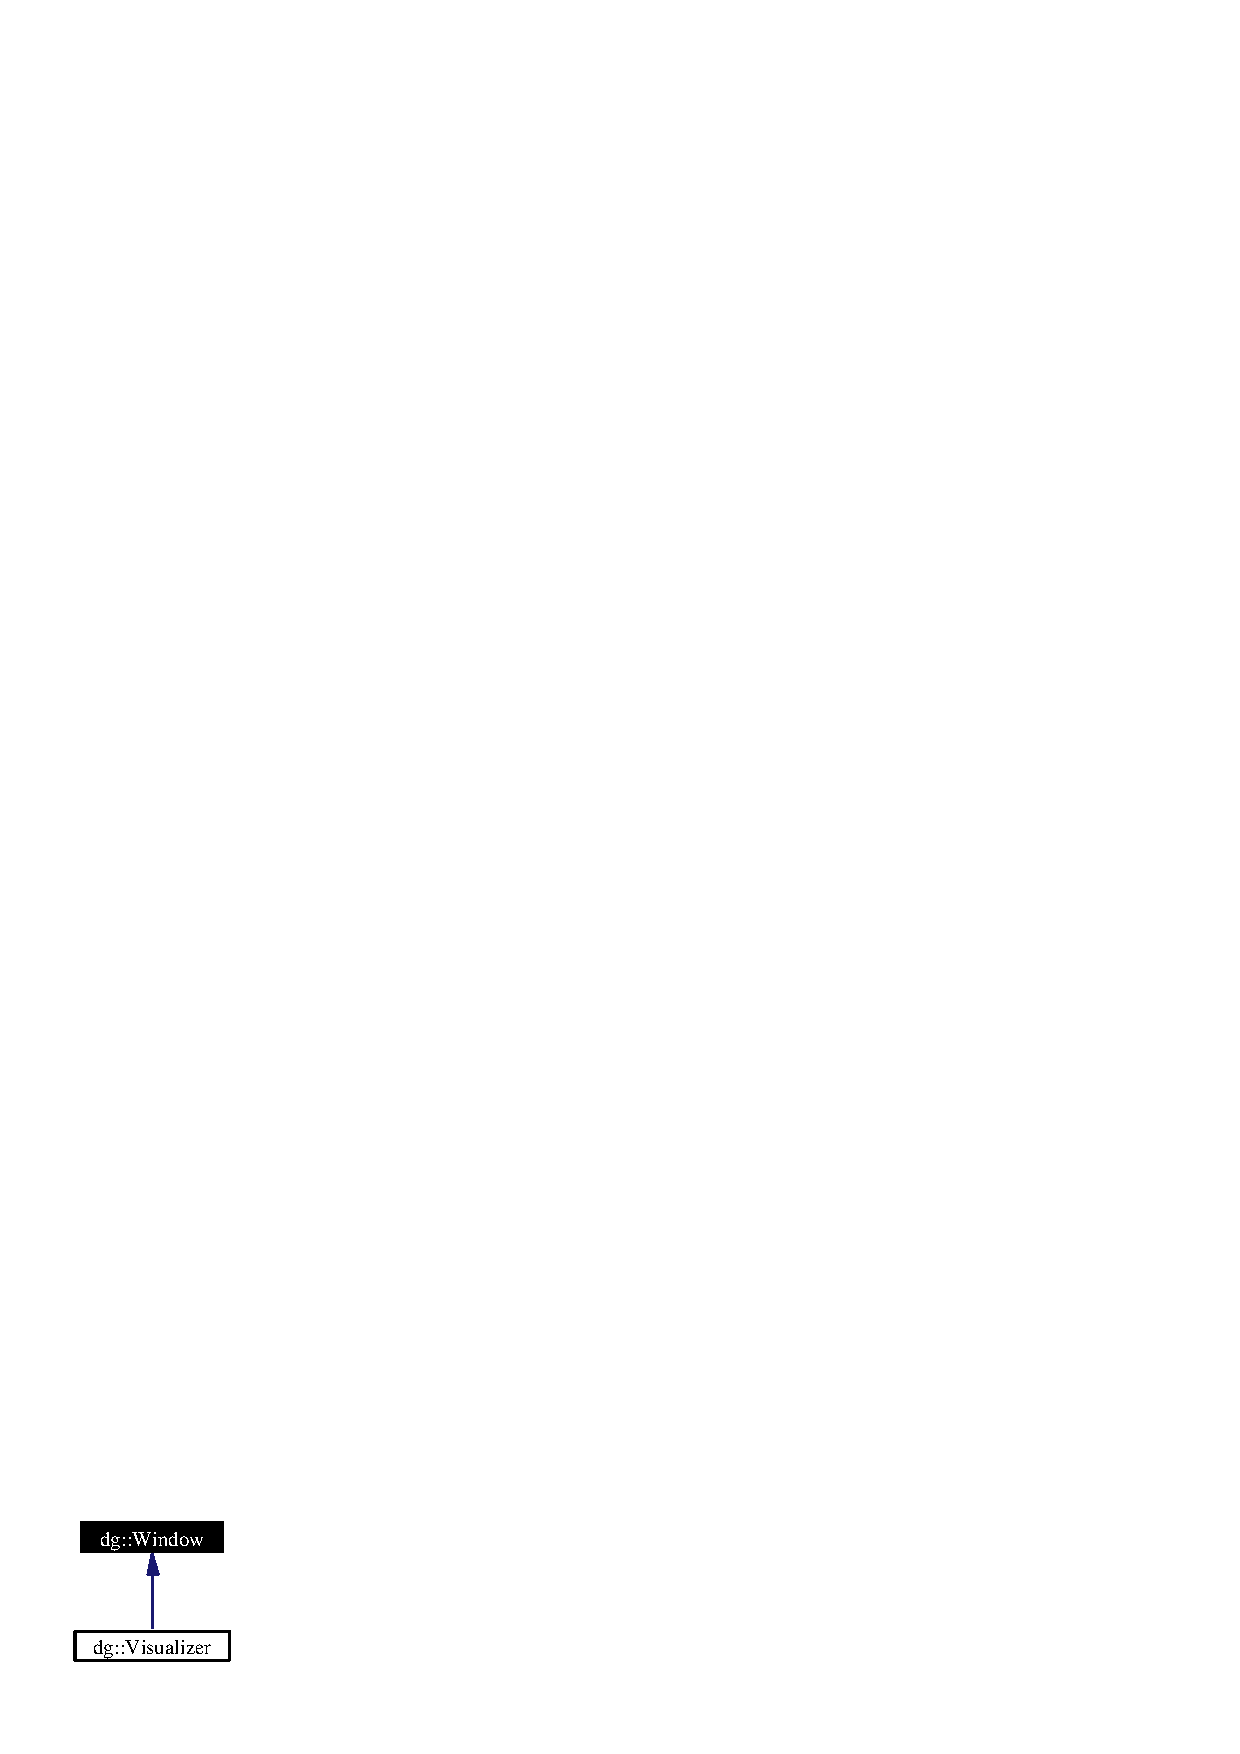
\includegraphics[width=55pt]{classdg_1_1Window__inherit__graph}
\end{center}
\end{figure}
Collaboration diagram for dg::Window:\begin{figure}[H]
\begin{center}
\leavevmode
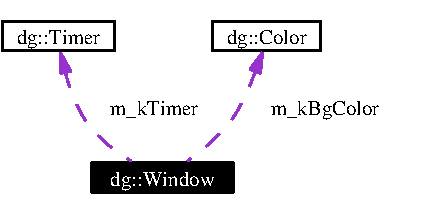
\includegraphics[width=119pt]{classdg_1_1Window__coll__graph}
\end{center}
\end{figure}
\subsection*{Public Methods}
\begin{CompactItemize}
\item 
virtual {\bf $\sim$Window} ()
\item 
virtual {\bf Bool} {\bf on\-Startup} ()
\item 
virtual {\bf Bool} {\bf on\-Initialize} ()
\item 
virtual void {\bf on\-Terminate} ()
\item 
virtual void {\bf on\-Move} ({\bf Int} i\-X, {\bf Int} i\-Y)
\item 
virtual void {\bf on\-Reshape} ({\bf Int} i\-Width, {\bf Int} i\-Height)
\item 
virtual void {\bf on\-Update} ({\bf Int} i\-Value)
\item 
virtual void {\bf on\-Display} ()
\item 
virtual void {\bf post\-Redisplay} ()
\item 
virtual void {\bf swap\-Buffers} ()
\item 
virtual void {\bf on\-Key\-Down} ({\bf UChar} uc\-Key, {\bf Int} i\-X, {\bf Int} i\-Y)
\item 
virtual void {\bf on\-Key\-Up} ({\bf UChar} uc\-Key, {\bf Int} i\-X, {\bf Int} i\-Y)
\item 
virtual void {\bf on\-Special\-Key\-Down} ({\bf Int} i\-Key, {\bf Int} i\-X, {\bf Int} i\-Y)
\item 
virtual void {\bf on\-Special\-Key\-Up} ({\bf Int} i\-Key, {\bf Int} i\-X, {\bf Int} i\-Y)
\item 
virtual void {\bf on\-Passive\-Motion} ({\bf Int} i\-X, {\bf Int} i\-Y)
\item 
virtual void {\bf on\-Mouse\-Motion} ({\bf Int} i\-X, {\bf Int} i\-Y, {\bf UInt} ui\-Modifiers)
\item 
virtual void {\bf on\-Mouse\-Click} ({\bf Int} i\-Button, {\bf Int} i\-State, {\bf Int} i\-X, {\bf Int} i\-Y, {\bf UInt} ui\-Modifiers)
\item 
virtual void {\bf on\-Idle} ()
\item 
void {\bf draw\-Image} (const {\bf UChar} $\ast$auc\-Buffer, {\bf UInt} ui\-Pos\-X, {\bf UInt} ui\-Pos\-Y, {\bf UInt} ui\-Width, {\bf UInt} ui\-Height, bool b\-Alpha)
\item 
void {\bf draw\-Image} (const {\bf Real} $\ast$af\-Buffer, {\bf UInt} ui\-Pos\-X, {\bf UInt} ui\-Pos\-Y, {\bf UInt} ui\-Width, {\bf UInt} ui\-Height, bool b\-Alpha)
\item 
void {\bf draw\-String} (const {\bf Char} $\ast$pc\-String, {\bf Int} i\-X, {\bf Int} i\-Y, const {\bf Color} \&rk\-Color)
\item 
void {\bf draw\-Frame\-Rate} ({\bf Int} i\-X, {\bf Int} i\-Y, const {\bf Color} \&rk\-Color)
\item 
void {\bf update\-Clicks} ()
\item 
void {\bf make\-Current} ()
\item 
char $\ast$ {\bf title} ()
\item 
{\bf UInt} {\bf x} ()
\item 
{\bf UInt} {\bf y} ()
\item 
{\bf UInt} {\bf width} ()
\item 
{\bf UInt} {\bf height} ()
\item 
const {\bf Color} \& {\bf bg} ()
\item 
{\bf Timer} \& {\bf timer} ()
\item 
void {\bf set\-Window\-ID} ({\bf Int} i\-Window\-ID)
\item 
{\bf Int} {\bf id} ()
\end{CompactItemize}
\subsection*{Static Public Methods}
\begin{CompactItemize}
\item 
Window $\ast$ {\bf current} ()
\end{CompactItemize}
\subsection*{Static Public Attributes}
\begin{CompactItemize}
\item 
const {\bf Int} {\bf KEY\_\-ESCAPE} = 0x1B
\item 
const {\bf Int} {\bf KEY\_\-LEFT\_\-ARROW} = GLUT\_\-KEY\_\-LEFT
\item 
const {\bf Int} {\bf KEY\_\-RIGHT\_\-ARROW} = GLUT\_\-KEY\_\-RIGHT
\item 
const {\bf Int} {\bf KEY\_\-UP\_\-ARROW} = GLUT\_\-KEY\_\-UP
\item 
const {\bf Int} {\bf KEY\_\-DOWN\_\-ARROW} = GLUT\_\-KEY\_\-DOWN
\item 
const {\bf Int} {\bf KEY\_\-HOME} = GLUT\_\-KEY\_\-HOME
\item 
const {\bf Int} {\bf KEY\_\-END} = GLUT\_\-KEY\_\-END
\item 
const {\bf Int} {\bf KEY\_\-PAGE\_\-UP} = GLUT\_\-KEY\_\-PAGE\_\-UP
\item 
const {\bf Int} {\bf KEY\_\-PAGE\_\-DOWN} = GLUT\_\-KEY\_\-PAGE\_\-DOWN
\item 
const {\bf Int} {\bf KEY\_\-INSERT} = GLUT\_\-KEY\_\-INSERT
\item 
const {\bf Int} {\bf KEY\_\-DELETE} = 0x2E
\item 
const {\bf Int} {\bf KEY\_\-F1} = GLUT\_\-KEY\_\-F1
\item 
const {\bf Int} {\bf KEY\_\-F2} = GLUT\_\-KEY\_\-F2
\item 
const {\bf Int} {\bf KEY\_\-F3} = GLUT\_\-KEY\_\-F3
\item 
const {\bf Int} {\bf KEY\_\-F4} = GLUT\_\-KEY\_\-F4
\item 
const {\bf Int} {\bf KEY\_\-F5} = GLUT\_\-KEY\_\-F5
\item 
const {\bf Int} {\bf KEY\_\-F6} = GLUT\_\-KEY\_\-F6
\item 
const {\bf Int} {\bf KEY\_\-F7} = GLUT\_\-KEY\_\-F7
\item 
const {\bf Int} {\bf KEY\_\-F8} = GLUT\_\-KEY\_\-F8
\item 
const {\bf Int} {\bf KEY\_\-F9} = GLUT\_\-KEY\_\-F9
\item 
const {\bf Int} {\bf KEY\_\-F10} = GLUT\_\-KEY\_\-F10
\item 
const {\bf Int} {\bf KEY\_\-F11} = GLUT\_\-KEY\_\-F11
\item 
const {\bf Int} {\bf KEY\_\-F12} = GLUT\_\-KEY\_\-F12
\item 
const {\bf Int} {\bf KEY\_\-SHIFT} = GLUT\_\-ACTIVE\_\-SHIFT
\item 
const {\bf Int} {\bf KEY\_\-CONTROL} = GLUT\_\-ACTIVE\_\-CTRL
\item 
const {\bf Int} {\bf KEY\_\-ALT} = GLUT\_\-ACTIVE\_\-ALT
\item 
const {\bf Int} {\bf KEY\_\-COMMAND} = 0
\item 
const {\bf Int} {\bf MOUSE\_\-LEFT\_\-BUTTON} = GLUT\_\-LEFT\_\-BUTTON
\item 
const {\bf Int} {\bf MOUSE\_\-MIDDLE\_\-BUTTON} = GLUT\_\-MIDDLE\_\-BUTTON
\item 
const {\bf Int} {\bf MOUSE\_\-RIGHT\_\-BUTTON} = GLUT\_\-RIGHT\_\-BUTTON
\item 
const {\bf Int} {\bf MOUSE\_\-UP} = GLUT\_\-UP
\item 
const {\bf Int} {\bf MOUSE\_\-DOWN} = GLUT\_\-DOWN
\item 
const {\bf Int} {\bf MOD\_\-LBUTTON}
\item 
const {\bf Int} {\bf MOD\_\-MBUTTON}
\item 
const {\bf Int} {\bf MOD\_\-RBUTTON}
\end{CompactItemize}
\subsection*{Protected Methods}
\begin{CompactItemize}
\item 
{\bf Window} (char $\ast$ac\-Window\-Title, {\bf Int} i\-X, {\bf Int} i\-Y, {\bf Int} i\-Width, {\bf Int} i\-Height, const {\bf Color} \&rk\-Bg\-Color)
\end{CompactItemize}
\subsection*{Protected Attributes}
\begin{CompactItemize}
\item 
{\bf Bool} {\bf m\_\-b\-Mouse\-Down}
\item 
{\bf Bool} {\bf m\_\-b\-Left\-Mouse\-Pressed}
\item 
{\bf Bool} {\bf m\_\-b\-Right\-Mouse\-Pressed}
\item 
{\bf Bool} {\bf m\_\-b\-Middle\-Mouse\-Pressed}
\item 
{\bf Int} {\bf m\_\-i\-Last\-Mouse\-X}
\item 
{\bf Int} {\bf m\_\-i\-Last\-Mouse\-Y}
\item 
{\bf Real} {\bf m\_\-f\-Frame\-Rate}
\item 
{\bf Int} {\bf m\_\-i\-Clicks}
\item 
{\bf Int} {\bf m\_\-i\-Timer}
\item 
{\bf Int} {\bf m\_\-i\-Max\-Timer}
\item 
char $\ast$ {\bf m\_\-ac\-Window\-Title}
\item 
{\bf Int} {\bf m\_\-i\-Window\-ID}
\item 
{\bf Int} {\bf m\_\-i\-X}
\item 
{\bf Int} {\bf m\_\-i\-Y}
\item 
{\bf Int} {\bf m\_\-i\-Width}
\item 
{\bf Int} {\bf m\_\-i\-Height}
\item 
{\bf Color} {\bf m\_\-k\-Bg\-Color}
\item 
{\bf Timer} {\bf m\_\-k\-Timer}
\end{CompactItemize}
\subsection*{Static Protected Attributes}
\begin{CompactItemize}
\item 
Window $\ast$ {\bf ms\_\-pk\-Window} = NULL
\end{CompactItemize}


\subsection{Constructor \& Destructor Documentation}
\index{dg::Window@{dg::Window}!~Window@{$\sim$Window}}
\index{~Window@{$\sim$Window}!dg::Window@{dg::Window}}
\subsubsection{\setlength{\rightskip}{0pt plus 5cm}Window::$\sim$Window ()\hspace{0.3cm}{\tt  [virtual]}}\label{classdg_1_1Window_a0}




Definition at line 27 of file Window.cpp.

References ms\_\-pk\-Window.\index{dg::Window@{dg::Window}!Window@{Window}}
\index{Window@{Window}!dg::Window@{dg::Window}}
\subsubsection{\setlength{\rightskip}{0pt plus 5cm}Window::Window (char $\ast$ {\em ac\-Window\-Title}, {\bf Int} {\em i\-X}, {\bf Int} {\em i\-Y}, {\bf Int} {\em i\-Width}, {\bf Int} {\em i\-Height}, const {\bf Color} \& {\em rk\-Bg\-Color})\hspace{0.3cm}{\tt  [protected]}}\label{classdg_1_1Window_b0}




Definition at line 9 of file Window.cpp.

References dg::Int, m\_\-ac\-Window\-Title, m\_\-i\-Clicks, m\_\-i\-Height, m\_\-i\-Max\-Timer, m\_\-i\-Timer, m\_\-i\-Width, m\_\-i\-X, m\_\-i\-Y, m\_\-k\-Bg\-Color, and ms\_\-pk\-Window.

\subsection{Member Function Documentation}
\index{dg::Window@{dg::Window}!bg@{bg}}
\index{bg@{bg}!dg::Window@{dg::Window}}
\subsubsection{\setlength{\rightskip}{0pt plus 5cm}const {\bf Color} \& dg::Window::bg ()\hspace{0.3cm}{\tt  [inline]}}\label{classdg_1_1Window_a29}




Definition at line 193 of file Window.h.

Referenced by dg::Visualizer::setup\-Ray\-Tracer().\index{dg::Window@{dg::Window}!current@{current}}
\index{current@{current}!dg::Window@{dg::Window}}
\subsubsection{\setlength{\rightskip}{0pt plus 5cm}Window $\ast$ dg::Window::current ()\hspace{0.3cm}{\tt  [inline, static]}}\label{classdg_1_1Window_d0}




Definition at line 163 of file Window.h.\index{dg::Window@{dg::Window}!drawFrameRate@{drawFrameRate}}
\index{drawFrameRate@{drawFrameRate}!dg::Window@{dg::Window}}
\subsubsection{\setlength{\rightskip}{0pt plus 5cm}void Window::draw\-Frame\-Rate ({\bf Int} {\em i\-X}, {\bf Int} {\em i\-Y}, const {\bf Color} \& {\em rk\-Color})}\label{classdg_1_1Window_a21}




Definition at line 132 of file Window.cpp.

References draw\-String(), dg::Timer::elapsed\-Seconds(), dg::Int, m\_\-f\-Frame\-Rate, m\_\-i\-Clicks, m\_\-i\-Max\-Timer, m\_\-i\-Timer, m\_\-k\-Timer, and dg::Real.\index{dg::Window@{dg::Window}!drawImage@{drawImage}}
\index{drawImage@{drawImage}!dg::Window@{dg::Window}}
\subsubsection{\setlength{\rightskip}{0pt plus 5cm}void Window::draw\-Image (const {\bf Real} $\ast$ {\em af\-Buffer}, {\bf UInt} {\em ui\-Pos\-X}, {\bf UInt} {\em ui\-Pos\-Y}, {\bf UInt} {\em ui\-Width}, {\bf UInt} {\em ui\-Height}, bool {\em b\-Alpha})}\label{classdg_1_1Window_a19}




Definition at line 209 of file Glut\-Window.cpp.

References m\_\-i\-Height, m\_\-i\-Width, dg::Real, and dg::UInt.\index{dg::Window@{dg::Window}!drawImage@{drawImage}}
\index{drawImage@{drawImage}!dg::Window@{dg::Window}}
\subsubsection{\setlength{\rightskip}{0pt plus 5cm}void Window::draw\-Image (const {\bf UChar} $\ast$ {\em auc\-Buffer}, {\bf UInt} {\em ui\-Pos\-X}, {\bf UInt} {\em ui\-Pos\-Y}, {\bf UInt} {\em ui\-Width}, {\bf UInt} {\em ui\-Height}, bool {\em b\-Alpha})}\label{classdg_1_1Window_a18}




Definition at line 147 of file Glut\-Window.cpp.

References m\_\-i\-Height, m\_\-i\-Width, dg::UChar, and dg::UInt.

Referenced by dg::Visualizer::draw\-Hypertexture(), and dg::Visualizer::draw\-Raytraced().\index{dg::Window@{dg::Window}!drawString@{drawString}}
\index{drawString@{drawString}!dg::Window@{dg::Window}}
\subsubsection{\setlength{\rightskip}{0pt plus 5cm}void Window::draw\-String (const {\bf Char} $\ast$ {\em pc\-String}, {\bf Int} {\em i\-X}, {\bf Int} {\em i\-Y}, const {\bf Color} \& {\em rk\-Color})}\label{classdg_1_1Window_a20}




Definition at line 131 of file Glut\-Window.cpp.

References dg::Color::a(), dg::Color::b(), dg::Char, dg::Color::g(), dg::Int, dg::Color::r(), and dg::UInt.

Referenced by draw\-Frame\-Rate(), and dg::Visualizer::draw\-Text().\index{dg::Window@{dg::Window}!height@{height}}
\index{height@{height}!dg::Window@{dg::Window}}
\subsubsection{\setlength{\rightskip}{0pt plus 5cm}{\bf UInt} dg::Window::height ()\hspace{0.3cm}{\tt  [inline]}}\label{classdg_1_1Window_a28}




Definition at line 188 of file Window.h.

Referenced by dg::Visualizer::draw\-Text(), dg::Visualizer::on\-Initialize(), dg::Visualizer::on\-Key\-Down(), dg::Visualizer::setup\-Camera(), dg::Visualizer::setup\-Hypertexture(), and dg::Visualizer::setup\-Ray\-Tracer().\index{dg::Window@{dg::Window}!id@{id}}
\index{id@{id}!dg::Window@{dg::Window}}
\subsubsection{\setlength{\rightskip}{0pt plus 5cm}{\bf Int} dg::Window::id ()\hspace{0.3cm}{\tt  [inline]}}\label{classdg_1_1Window_a32}




Definition at line 203 of file Window.h.

Referenced by make\-Current(), and post\-Redisplay().\index{dg::Window@{dg::Window}!makeCurrent@{makeCurrent}}
\index{makeCurrent@{makeCurrent}!dg::Window@{dg::Window}}
\subsubsection{\setlength{\rightskip}{0pt plus 5cm}void Window::make\-Current ()}\label{classdg_1_1Window_a23}




Definition at line 115 of file Glut\-Window.cpp.

References id(), and ms\_\-pk\-Window.\index{dg::Window@{dg::Window}!onDisplay@{onDisplay}}
\index{onDisplay@{onDisplay}!dg::Window@{dg::Window}}
\subsubsection{\setlength{\rightskip}{0pt plus 5cm}void Window::on\-Display ()\hspace{0.3cm}{\tt  [virtual]}}\label{classdg_1_1Window_a7}




Reimplemented in {\bf dg::Visualizer} {\rm (p.\,\pageref{classdg_1_1Visualizer_a5})}.

Definition at line 55 of file Window.cpp.

Referenced by on\-Idle().\index{dg::Window@{dg::Window}!onIdle@{onIdle}}
\index{onIdle@{onIdle}!dg::Window@{dg::Window}}
\subsubsection{\setlength{\rightskip}{0pt plus 5cm}void Window::on\-Idle ()\hspace{0.3cm}{\tt  [virtual]}}\label{classdg_1_1Window_a17}




Reimplemented in {\bf dg::Visualizer} {\rm (p.\,\pageref{classdg_1_1Visualizer_a6})}.

Definition at line 60 of file Window.cpp.

References on\-Display().\index{dg::Window@{dg::Window}!onInitialize@{onInitialize}}
\index{onInitialize@{onInitialize}!dg::Window@{dg::Window}}
\subsubsection{\setlength{\rightskip}{0pt plus 5cm}{\bf Bool} Window::on\-Initialize ()\hspace{0.3cm}{\tt  [virtual]}}\label{classdg_1_1Window_a2}




Reimplemented in {\bf dg::Visualizer} {\rm (p.\,\pageref{classdg_1_1Visualizer_a3})}.

Definition at line 38 of file Window.cpp.

References dg::Bool.\index{dg::Window@{dg::Window}!onKeyDown@{onKeyDown}}
\index{onKeyDown@{onKeyDown}!dg::Window@{dg::Window}}
\subsubsection{\setlength{\rightskip}{0pt plus 5cm}void Window::on\-Key\-Down ({\bf UChar} {\em uc\-Key}, {\bf Int} {\em i\-X}, {\bf Int} {\em i\-Y})\hspace{0.3cm}{\tt  [virtual]}}\label{classdg_1_1Window_a10}




Reimplemented in {\bf dg::Visualizer} {\rm (p.\,\pageref{classdg_1_1Visualizer_a7})}.

Definition at line 65 of file Window.cpp.

References dg::Int, KEY\_\-ESCAPE, on\-Terminate(), and dg::UChar.\index{dg::Window@{dg::Window}!onKeyUp@{onKeyUp}}
\index{onKeyUp@{onKeyUp}!dg::Window@{dg::Window}}
\subsubsection{\setlength{\rightskip}{0pt plus 5cm}void Window::on\-Key\-Up ({\bf UChar} {\em uc\-Key}, {\bf Int} {\em i\-X}, {\bf Int} {\em i\-Y})\hspace{0.3cm}{\tt  [virtual]}}\label{classdg_1_1Window_a11}




Definition at line 72 of file Window.cpp.

References dg::Int, and dg::UChar.\index{dg::Window@{dg::Window}!onMouseClick@{onMouseClick}}
\index{onMouseClick@{onMouseClick}!dg::Window@{dg::Window}}
\subsubsection{\setlength{\rightskip}{0pt plus 5cm}void Window::on\-Mouse\-Click ({\bf Int} {\em i\-Button}, {\bf Int} {\em i\-State}, {\bf Int} {\em i\-X}, {\bf Int} {\em i\-Y}, {\bf UInt} {\em ui\-Modifiers})\hspace{0.3cm}{\tt  [virtual]}}\label{classdg_1_1Window_a16}




Reimplemented in {\bf dg::Visualizer} {\rm (p.\,\pageref{classdg_1_1Visualizer_a10})}.

Definition at line 87 of file Window.cpp.

References dg::Int, m\_\-b\-Left\-Mouse\-Pressed, m\_\-b\-Middle\-Mouse\-Pressed, m\_\-b\-Mouse\-Down, m\_\-b\-Right\-Mouse\-Pressed, m\_\-i\-Last\-Mouse\-X, m\_\-i\-Last\-Mouse\-Y, and dg::UInt.\index{dg::Window@{dg::Window}!onMouseMotion@{onMouseMotion}}
\index{onMouseMotion@{onMouseMotion}!dg::Window@{dg::Window}}
\subsubsection{\setlength{\rightskip}{0pt plus 5cm}void Window::on\-Mouse\-Motion ({\bf Int} {\em i\-X}, {\bf Int} {\em i\-Y}, {\bf UInt} {\em ui\-Modifiers})\hspace{0.3cm}{\tt  [virtual]}}\label{classdg_1_1Window_a15}




Reimplemented in {\bf dg::Visualizer} {\rm (p.\,\pageref{classdg_1_1Visualizer_a9})}.

Definition at line 115 of file Window.cpp.

References dg::Int, and dg::UInt.\index{dg::Window@{dg::Window}!onMove@{onMove}}
\index{onMove@{onMove}!dg::Window@{dg::Window}}
\subsubsection{\setlength{\rightskip}{0pt plus 5cm}void Window::on\-Move ({\bf Int} {\em i\-X}, {\bf Int} {\em i\-Y})\hspace{0.3cm}{\tt  [virtual]}}\label{classdg_1_1Window_a4}




Definition at line 43 of file Window.cpp.

References dg::Int, m\_\-i\-X, and m\_\-i\-Y.\index{dg::Window@{dg::Window}!onPassiveMotion@{onPassiveMotion}}
\index{onPassiveMotion@{onPassiveMotion}!dg::Window@{dg::Window}}
\subsubsection{\setlength{\rightskip}{0pt plus 5cm}void Window::on\-Passive\-Motion ({\bf Int} {\em i\-X}, {\bf Int} {\em i\-Y})\hspace{0.3cm}{\tt  [virtual]}}\label{classdg_1_1Window_a14}




Definition at line 120 of file Window.cpp.

References dg::Int.\index{dg::Window@{dg::Window}!onReshape@{onReshape}}
\index{onReshape@{onReshape}!dg::Window@{dg::Window}}
\subsubsection{\setlength{\rightskip}{0pt plus 5cm}void Window::on\-Reshape ({\bf Int} {\em i\-Width}, {\bf Int} {\em i\-Height})\hspace{0.3cm}{\tt  [virtual]}}\label{classdg_1_1Window_a5}




Reimplemented in {\bf dg::Visualizer} {\rm (p.\,\pageref{classdg_1_1Visualizer_a4})}.

Definition at line 49 of file Window.cpp.

References dg::Int, m\_\-i\-Height, and m\_\-i\-Width.\index{dg::Window@{dg::Window}!onSpecialKeyDown@{onSpecialKeyDown}}
\index{onSpecialKeyDown@{onSpecialKeyDown}!dg::Window@{dg::Window}}
\subsubsection{\setlength{\rightskip}{0pt plus 5cm}void Window::on\-Special\-Key\-Down ({\bf Int} {\em i\-Key}, {\bf Int} {\em i\-X}, {\bf Int} {\em i\-Y})\hspace{0.3cm}{\tt  [virtual]}}\label{classdg_1_1Window_a12}




Reimplemented in {\bf dg::Visualizer} {\rm (p.\,\pageref{classdg_1_1Visualizer_a8})}.

Definition at line 77 of file Window.cpp.

References dg::Int.\index{dg::Window@{dg::Window}!onSpecialKeyUp@{onSpecialKeyUp}}
\index{onSpecialKeyUp@{onSpecialKeyUp}!dg::Window@{dg::Window}}
\subsubsection{\setlength{\rightskip}{0pt plus 5cm}void Window::on\-Special\-Key\-Up ({\bf Int} {\em i\-Key}, {\bf Int} {\em i\-X}, {\bf Int} {\em i\-Y})\hspace{0.3cm}{\tt  [virtual]}}\label{classdg_1_1Window_a13}




Definition at line 82 of file Window.cpp.

References dg::Int.\index{dg::Window@{dg::Window}!onStartup@{onStartup}}
\index{onStartup@{onStartup}!dg::Window@{dg::Window}}
\subsubsection{\setlength{\rightskip}{0pt plus 5cm}{\bf Bool} Window::on\-Startup ()\hspace{0.3cm}{\tt  [virtual]}}\label{classdg_1_1Window_a1}




Reimplemented in {\bf dg::Visualizer} {\rm (p.\,\pageref{classdg_1_1Visualizer_a2})}.

Definition at line 33 of file Window.cpp.

References dg::Bool.\index{dg::Window@{dg::Window}!onTerminate@{onTerminate}}
\index{onTerminate@{onTerminate}!dg::Window@{dg::Window}}
\subsubsection{\setlength{\rightskip}{0pt plus 5cm}void Window::on\-Terminate ()\hspace{0.3cm}{\tt  [virtual]}}\label{classdg_1_1Window_a3}




Definition at line 101 of file Glut\-Window.cpp.

Referenced by on\-Key\-Down().\index{dg::Window@{dg::Window}!onUpdate@{onUpdate}}
\index{onUpdate@{onUpdate}!dg::Window@{dg::Window}}
\subsubsection{\setlength{\rightskip}{0pt plus 5cm}void Window::on\-Update ({\bf Int} {\em i\-Value})\hspace{0.3cm}{\tt  [virtual]}}\label{classdg_1_1Window_a6}




Definition at line 107 of file Glut\-Window.cpp.

References dg::Int, and post\-Redisplay().\index{dg::Window@{dg::Window}!postRedisplay@{postRedisplay}}
\index{postRedisplay@{postRedisplay}!dg::Window@{dg::Window}}
\subsubsection{\setlength{\rightskip}{0pt plus 5cm}void Window::post\-Redisplay ()\hspace{0.3cm}{\tt  [virtual]}}\label{classdg_1_1Window_a8}




Definition at line 121 of file Glut\-Window.cpp.

References id().

Referenced by dg::Visualizer::draw\-Hypertexture(), dg::Visualizer::draw\-Raytraced(), on\-Update(), dg::Visualizer::setup\-Hypertexture(), dg::Visualizer::setup\-Polygonizer(), and dg::Visualizer::setup\-Ray\-Tracer().\index{dg::Window@{dg::Window}!setWindowID@{setWindowID}}
\index{setWindowID@{setWindowID}!dg::Window@{dg::Window}}
\subsubsection{\setlength{\rightskip}{0pt plus 5cm}void dg::Window::set\-Window\-ID ({\bf Int} {\em i\-Window\-ID})\hspace{0.3cm}{\tt  [inline]}}\label{classdg_1_1Window_a31}




Definition at line 198 of file Window.h.\index{dg::Window@{dg::Window}!swapBuffers@{swapBuffers}}
\index{swapBuffers@{swapBuffers}!dg::Window@{dg::Window}}
\subsubsection{\setlength{\rightskip}{0pt plus 5cm}void Window::swap\-Buffers ()\hspace{0.3cm}{\tt  [virtual]}}\label{classdg_1_1Window_a9}




Definition at line 126 of file Glut\-Window.cpp.

Referenced by dg::Visualizer::draw\-Hypertexture(), dg::Visualizer::draw\-Raytraced(), and dg::Visualizer::on\-Display().\index{dg::Window@{dg::Window}!timer@{timer}}
\index{timer@{timer}!dg::Window@{dg::Window}}
\subsubsection{\setlength{\rightskip}{0pt plus 5cm}{\bf Timer} \& dg::Window::timer ()\hspace{0.3cm}{\tt  [inline]}}\label{classdg_1_1Window_a30}




Definition at line 208 of file Window.h.\index{dg::Window@{dg::Window}!title@{title}}
\index{title@{title}!dg::Window@{dg::Window}}
\subsubsection{\setlength{\rightskip}{0pt plus 5cm}char $\ast$ dg::Window::title ()\hspace{0.3cm}{\tt  [inline]}}\label{classdg_1_1Window_a24}




Definition at line 168 of file Window.h.\index{dg::Window@{dg::Window}!updateClicks@{updateClicks}}
\index{updateClicks@{updateClicks}!dg::Window@{dg::Window}}
\subsubsection{\setlength{\rightskip}{0pt plus 5cm}void Window::update\-Clicks ()}\label{classdg_1_1Window_a22}




Definition at line 125 of file Window.cpp.

References m\_\-i\-Clicks.

Referenced by dg::Visualizer::on\-Display().\index{dg::Window@{dg::Window}!width@{width}}
\index{width@{width}!dg::Window@{dg::Window}}
\subsubsection{\setlength{\rightskip}{0pt plus 5cm}{\bf UInt} dg::Window::width ()\hspace{0.3cm}{\tt  [inline]}}\label{classdg_1_1Window_a27}




Definition at line 183 of file Window.h.

Referenced by dg::Visualizer::draw\-Text(), dg::Visualizer::on\-Initialize(), dg::Visualizer::on\-Key\-Down(), dg::Visualizer::setup\-Camera(), dg::Visualizer::setup\-Hypertexture(), and dg::Visualizer::setup\-Ray\-Tracer().\index{dg::Window@{dg::Window}!x@{x}}
\index{x@{x}!dg::Window@{dg::Window}}
\subsubsection{\setlength{\rightskip}{0pt plus 5cm}{\bf UInt} dg::Window::x ()\hspace{0.3cm}{\tt  [inline]}}\label{classdg_1_1Window_a25}




Definition at line 173 of file Window.h.\index{dg::Window@{dg::Window}!y@{y}}
\index{y@{y}!dg::Window@{dg::Window}}
\subsubsection{\setlength{\rightskip}{0pt plus 5cm}{\bf UInt} dg::Window::y ()\hspace{0.3cm}{\tt  [inline]}}\label{classdg_1_1Window_a26}




Definition at line 178 of file Window.h.

\subsection{Member Data Documentation}
\index{dg::Window@{dg::Window}!KEY_ALT@{KEY\_\-ALT}}
\index{KEY_ALT@{KEY\_\-ALT}!dg::Window@{dg::Window}}
\subsubsection{\setlength{\rightskip}{0pt plus 5cm}const {\bf Int} Window::KEY\_\-ALT = GLUT\_\-ACTIVE\_\-ALT\hspace{0.3cm}{\tt  [static]}}\label{classdg_1_1Window_p25}




Definition at line 34 of file Glut\-Key\-Bindings.h.\index{dg::Window@{dg::Window}!KEY_COMMAND@{KEY\_\-COMMAND}}
\index{KEY_COMMAND@{KEY\_\-COMMAND}!dg::Window@{dg::Window}}
\subsubsection{\setlength{\rightskip}{0pt plus 5cm}const {\bf Int} Window::KEY\_\-COMMAND = 0\hspace{0.3cm}{\tt  [static]}}\label{classdg_1_1Window_p26}




Definition at line 35 of file Glut\-Key\-Bindings.h.\index{dg::Window@{dg::Window}!KEY_CONTROL@{KEY\_\-CONTROL}}
\index{KEY_CONTROL@{KEY\_\-CONTROL}!dg::Window@{dg::Window}}
\subsubsection{\setlength{\rightskip}{0pt plus 5cm}const {\bf Int} Window::KEY\_\-CONTROL = GLUT\_\-ACTIVE\_\-CTRL\hspace{0.3cm}{\tt  [static]}}\label{classdg_1_1Window_p24}




Definition at line 33 of file Glut\-Key\-Bindings.h.\index{dg::Window@{dg::Window}!KEY_DELETE@{KEY\_\-DELETE}}
\index{KEY_DELETE@{KEY\_\-DELETE}!dg::Window@{dg::Window}}
\subsubsection{\setlength{\rightskip}{0pt plus 5cm}const {\bf Int} Window::KEY\_\-DELETE = 0x2E\hspace{0.3cm}{\tt  [static]}}\label{classdg_1_1Window_p10}




Definition at line 18 of file Glut\-Key\-Bindings.h.\index{dg::Window@{dg::Window}!KEY_DOWN_ARROW@{KEY\_\-DOWN\_\-ARROW}}
\index{KEY_DOWN_ARROW@{KEY\_\-DOWN\_\-ARROW}!dg::Window@{dg::Window}}
\subsubsection{\setlength{\rightskip}{0pt plus 5cm}const {\bf Int} Window::KEY\_\-DOWN\_\-ARROW = GLUT\_\-KEY\_\-DOWN\hspace{0.3cm}{\tt  [static]}}\label{classdg_1_1Window_p4}




Definition at line 12 of file Glut\-Key\-Bindings.h.\index{dg::Window@{dg::Window}!KEY_END@{KEY\_\-END}}
\index{KEY_END@{KEY\_\-END}!dg::Window@{dg::Window}}
\subsubsection{\setlength{\rightskip}{0pt plus 5cm}const {\bf Int} Window::KEY\_\-END = GLUT\_\-KEY\_\-END\hspace{0.3cm}{\tt  [static]}}\label{classdg_1_1Window_p6}




Definition at line 14 of file Glut\-Key\-Bindings.h.\index{dg::Window@{dg::Window}!KEY_ESCAPE@{KEY\_\-ESCAPE}}
\index{KEY_ESCAPE@{KEY\_\-ESCAPE}!dg::Window@{dg::Window}}
\subsubsection{\setlength{\rightskip}{0pt plus 5cm}const {\bf Int} Window::KEY\_\-ESCAPE = 0x1B\hspace{0.3cm}{\tt  [static]}}\label{classdg_1_1Window_p0}




Definition at line 8 of file Glut\-Key\-Bindings.h.

Referenced by on\-Key\-Down().\index{dg::Window@{dg::Window}!KEY_F1@{KEY\_\-F1}}
\index{KEY_F1@{KEY\_\-F1}!dg::Window@{dg::Window}}
\subsubsection{\setlength{\rightskip}{0pt plus 5cm}const {\bf Int} Window::KEY\_\-F1 = GLUT\_\-KEY\_\-F1\hspace{0.3cm}{\tt  [static]}}\label{classdg_1_1Window_p11}




Definition at line 19 of file Glut\-Key\-Bindings.h.\index{dg::Window@{dg::Window}!KEY_F10@{KEY\_\-F10}}
\index{KEY_F10@{KEY\_\-F10}!dg::Window@{dg::Window}}
\subsubsection{\setlength{\rightskip}{0pt plus 5cm}const {\bf Int} Window::KEY\_\-F10 = GLUT\_\-KEY\_\-F10\hspace{0.3cm}{\tt  [static]}}\label{classdg_1_1Window_p20}




Definition at line 28 of file Glut\-Key\-Bindings.h.\index{dg::Window@{dg::Window}!KEY_F11@{KEY\_\-F11}}
\index{KEY_F11@{KEY\_\-F11}!dg::Window@{dg::Window}}
\subsubsection{\setlength{\rightskip}{0pt plus 5cm}const {\bf Int} Window::KEY\_\-F11 = GLUT\_\-KEY\_\-F11\hspace{0.3cm}{\tt  [static]}}\label{classdg_1_1Window_p21}




Definition at line 29 of file Glut\-Key\-Bindings.h.\index{dg::Window@{dg::Window}!KEY_F12@{KEY\_\-F12}}
\index{KEY_F12@{KEY\_\-F12}!dg::Window@{dg::Window}}
\subsubsection{\setlength{\rightskip}{0pt plus 5cm}const {\bf Int} Window::KEY\_\-F12 = GLUT\_\-KEY\_\-F12\hspace{0.3cm}{\tt  [static]}}\label{classdg_1_1Window_p22}




Definition at line 30 of file Glut\-Key\-Bindings.h.\index{dg::Window@{dg::Window}!KEY_F2@{KEY\_\-F2}}
\index{KEY_F2@{KEY\_\-F2}!dg::Window@{dg::Window}}
\subsubsection{\setlength{\rightskip}{0pt plus 5cm}const {\bf Int} Window::KEY\_\-F2 = GLUT\_\-KEY\_\-F2\hspace{0.3cm}{\tt  [static]}}\label{classdg_1_1Window_p12}




Definition at line 20 of file Glut\-Key\-Bindings.h.\index{dg::Window@{dg::Window}!KEY_F3@{KEY\_\-F3}}
\index{KEY_F3@{KEY\_\-F3}!dg::Window@{dg::Window}}
\subsubsection{\setlength{\rightskip}{0pt plus 5cm}const {\bf Int} Window::KEY\_\-F3 = GLUT\_\-KEY\_\-F3\hspace{0.3cm}{\tt  [static]}}\label{classdg_1_1Window_p13}




Definition at line 21 of file Glut\-Key\-Bindings.h.\index{dg::Window@{dg::Window}!KEY_F4@{KEY\_\-F4}}
\index{KEY_F4@{KEY\_\-F4}!dg::Window@{dg::Window}}
\subsubsection{\setlength{\rightskip}{0pt plus 5cm}const {\bf Int} Window::KEY\_\-F4 = GLUT\_\-KEY\_\-F4\hspace{0.3cm}{\tt  [static]}}\label{classdg_1_1Window_p14}




Definition at line 22 of file Glut\-Key\-Bindings.h.\index{dg::Window@{dg::Window}!KEY_F5@{KEY\_\-F5}}
\index{KEY_F5@{KEY\_\-F5}!dg::Window@{dg::Window}}
\subsubsection{\setlength{\rightskip}{0pt plus 5cm}const {\bf Int} Window::KEY\_\-F5 = GLUT\_\-KEY\_\-F5\hspace{0.3cm}{\tt  [static]}}\label{classdg_1_1Window_p15}




Definition at line 23 of file Glut\-Key\-Bindings.h.\index{dg::Window@{dg::Window}!KEY_F6@{KEY\_\-F6}}
\index{KEY_F6@{KEY\_\-F6}!dg::Window@{dg::Window}}
\subsubsection{\setlength{\rightskip}{0pt plus 5cm}const {\bf Int} Window::KEY\_\-F6 = GLUT\_\-KEY\_\-F6\hspace{0.3cm}{\tt  [static]}}\label{classdg_1_1Window_p16}




Definition at line 24 of file Glut\-Key\-Bindings.h.\index{dg::Window@{dg::Window}!KEY_F7@{KEY\_\-F7}}
\index{KEY_F7@{KEY\_\-F7}!dg::Window@{dg::Window}}
\subsubsection{\setlength{\rightskip}{0pt plus 5cm}const {\bf Int} Window::KEY\_\-F7 = GLUT\_\-KEY\_\-F7\hspace{0.3cm}{\tt  [static]}}\label{classdg_1_1Window_p17}




Definition at line 25 of file Glut\-Key\-Bindings.h.\index{dg::Window@{dg::Window}!KEY_F8@{KEY\_\-F8}}
\index{KEY_F8@{KEY\_\-F8}!dg::Window@{dg::Window}}
\subsubsection{\setlength{\rightskip}{0pt plus 5cm}const {\bf Int} Window::KEY\_\-F8 = GLUT\_\-KEY\_\-F8\hspace{0.3cm}{\tt  [static]}}\label{classdg_1_1Window_p18}




Definition at line 26 of file Glut\-Key\-Bindings.h.\index{dg::Window@{dg::Window}!KEY_F9@{KEY\_\-F9}}
\index{KEY_F9@{KEY\_\-F9}!dg::Window@{dg::Window}}
\subsubsection{\setlength{\rightskip}{0pt plus 5cm}const {\bf Int} Window::KEY\_\-F9 = GLUT\_\-KEY\_\-F9\hspace{0.3cm}{\tt  [static]}}\label{classdg_1_1Window_p19}




Definition at line 27 of file Glut\-Key\-Bindings.h.\index{dg::Window@{dg::Window}!KEY_HOME@{KEY\_\-HOME}}
\index{KEY_HOME@{KEY\_\-HOME}!dg::Window@{dg::Window}}
\subsubsection{\setlength{\rightskip}{0pt plus 5cm}const {\bf Int} Window::KEY\_\-HOME = GLUT\_\-KEY\_\-HOME\hspace{0.3cm}{\tt  [static]}}\label{classdg_1_1Window_p5}




Definition at line 13 of file Glut\-Key\-Bindings.h.\index{dg::Window@{dg::Window}!KEY_INSERT@{KEY\_\-INSERT}}
\index{KEY_INSERT@{KEY\_\-INSERT}!dg::Window@{dg::Window}}
\subsubsection{\setlength{\rightskip}{0pt plus 5cm}const {\bf Int} Window::KEY\_\-INSERT = GLUT\_\-KEY\_\-INSERT\hspace{0.3cm}{\tt  [static]}}\label{classdg_1_1Window_p9}




Definition at line 17 of file Glut\-Key\-Bindings.h.\index{dg::Window@{dg::Window}!KEY_LEFT_ARROW@{KEY\_\-LEFT\_\-ARROW}}
\index{KEY_LEFT_ARROW@{KEY\_\-LEFT\_\-ARROW}!dg::Window@{dg::Window}}
\subsubsection{\setlength{\rightskip}{0pt plus 5cm}const {\bf Int} Window::KEY\_\-LEFT\_\-ARROW = GLUT\_\-KEY\_\-LEFT\hspace{0.3cm}{\tt  [static]}}\label{classdg_1_1Window_p1}




Definition at line 9 of file Glut\-Key\-Bindings.h.\index{dg::Window@{dg::Window}!KEY_PAGE_DOWN@{KEY\_\-PAGE\_\-DOWN}}
\index{KEY_PAGE_DOWN@{KEY\_\-PAGE\_\-DOWN}!dg::Window@{dg::Window}}
\subsubsection{\setlength{\rightskip}{0pt plus 5cm}const {\bf Int} Window::KEY\_\-PAGE\_\-DOWN = GLUT\_\-KEY\_\-PAGE\_\-DOWN\hspace{0.3cm}{\tt  [static]}}\label{classdg_1_1Window_p8}




Definition at line 16 of file Glut\-Key\-Bindings.h.\index{dg::Window@{dg::Window}!KEY_PAGE_UP@{KEY\_\-PAGE\_\-UP}}
\index{KEY_PAGE_UP@{KEY\_\-PAGE\_\-UP}!dg::Window@{dg::Window}}
\subsubsection{\setlength{\rightskip}{0pt plus 5cm}const {\bf Int} Window::KEY\_\-PAGE\_\-UP = GLUT\_\-KEY\_\-PAGE\_\-UP\hspace{0.3cm}{\tt  [static]}}\label{classdg_1_1Window_p7}




Definition at line 15 of file Glut\-Key\-Bindings.h.\index{dg::Window@{dg::Window}!KEY_RIGHT_ARROW@{KEY\_\-RIGHT\_\-ARROW}}
\index{KEY_RIGHT_ARROW@{KEY\_\-RIGHT\_\-ARROW}!dg::Window@{dg::Window}}
\subsubsection{\setlength{\rightskip}{0pt plus 5cm}const {\bf Int} Window::KEY\_\-RIGHT\_\-ARROW = GLUT\_\-KEY\_\-RIGHT\hspace{0.3cm}{\tt  [static]}}\label{classdg_1_1Window_p2}




Definition at line 10 of file Glut\-Key\-Bindings.h.\index{dg::Window@{dg::Window}!KEY_SHIFT@{KEY\_\-SHIFT}}
\index{KEY_SHIFT@{KEY\_\-SHIFT}!dg::Window@{dg::Window}}
\subsubsection{\setlength{\rightskip}{0pt plus 5cm}const {\bf Int} Window::KEY\_\-SHIFT = GLUT\_\-ACTIVE\_\-SHIFT\hspace{0.3cm}{\tt  [static]}}\label{classdg_1_1Window_p23}




Definition at line 32 of file Glut\-Key\-Bindings.h.\index{dg::Window@{dg::Window}!KEY_UP_ARROW@{KEY\_\-UP\_\-ARROW}}
\index{KEY_UP_ARROW@{KEY\_\-UP\_\-ARROW}!dg::Window@{dg::Window}}
\subsubsection{\setlength{\rightskip}{0pt plus 5cm}const {\bf Int} Window::KEY\_\-UP\_\-ARROW = GLUT\_\-KEY\_\-UP\hspace{0.3cm}{\tt  [static]}}\label{classdg_1_1Window_p3}




Definition at line 11 of file Glut\-Key\-Bindings.h.\index{dg::Window@{dg::Window}!m_acWindowTitle@{m\_\-acWindowTitle}}
\index{m_acWindowTitle@{m\_\-acWindowTitle}!dg::Window@{dg::Window}}
\subsubsection{\setlength{\rightskip}{0pt plus 5cm}char$\ast$ dg::Window::m\_\-ac\-Window\-Title\hspace{0.3cm}{\tt  [protected]}}\label{classdg_1_1Window_n10}




Definition at line 152 of file Window.h.

Referenced by Window().\index{dg::Window@{dg::Window}!m_bLeftMousePressed@{m\_\-bLeftMousePressed}}
\index{m_bLeftMousePressed@{m\_\-bLeftMousePressed}!dg::Window@{dg::Window}}
\subsubsection{\setlength{\rightskip}{0pt plus 5cm}{\bf Bool} dg::Window::m\_\-b\-Left\-Mouse\-Pressed\hspace{0.3cm}{\tt  [protected]}}\label{classdg_1_1Window_n1}




Definition at line 138 of file Window.h.

Referenced by on\-Mouse\-Click(), and dg::Visualizer::on\-Mouse\-Click().\index{dg::Window@{dg::Window}!m_bMiddleMousePressed@{m\_\-bMiddleMousePressed}}
\index{m_bMiddleMousePressed@{m\_\-bMiddleMousePressed}!dg::Window@{dg::Window}}
\subsubsection{\setlength{\rightskip}{0pt plus 5cm}{\bf Bool} dg::Window::m\_\-b\-Middle\-Mouse\-Pressed\hspace{0.3cm}{\tt  [protected]}}\label{classdg_1_1Window_n3}




Definition at line 140 of file Window.h.

Referenced by on\-Mouse\-Click(), and dg::Visualizer::on\-Mouse\-Click().\index{dg::Window@{dg::Window}!m_bMouseDown@{m\_\-bMouseDown}}
\index{m_bMouseDown@{m\_\-bMouseDown}!dg::Window@{dg::Window}}
\subsubsection{\setlength{\rightskip}{0pt plus 5cm}{\bf Bool} dg::Window::m\_\-b\-Mouse\-Down\hspace{0.3cm}{\tt  [protected]}}\label{classdg_1_1Window_n0}




Definition at line 137 of file Window.h.

Referenced by on\-Mouse\-Click().\index{dg::Window@{dg::Window}!m_bRightMousePressed@{m\_\-bRightMousePressed}}
\index{m_bRightMousePressed@{m\_\-bRightMousePressed}!dg::Window@{dg::Window}}
\subsubsection{\setlength{\rightskip}{0pt plus 5cm}{\bf Bool} dg::Window::m\_\-b\-Right\-Mouse\-Pressed\hspace{0.3cm}{\tt  [protected]}}\label{classdg_1_1Window_n2}




Definition at line 139 of file Window.h.

Referenced by on\-Mouse\-Click(), and dg::Visualizer::on\-Mouse\-Click().\index{dg::Window@{dg::Window}!m_fFrameRate@{m\_\-fFrameRate}}
\index{m_fFrameRate@{m\_\-fFrameRate}!dg::Window@{dg::Window}}
\subsubsection{\setlength{\rightskip}{0pt plus 5cm}{\bf Real} dg::Window::m\_\-f\-Frame\-Rate\hspace{0.3cm}{\tt  [protected]}}\label{classdg_1_1Window_n6}




Definition at line 145 of file Window.h.

Referenced by draw\-Frame\-Rate().\index{dg::Window@{dg::Window}!m_iClicks@{m\_\-iClicks}}
\index{m_iClicks@{m\_\-iClicks}!dg::Window@{dg::Window}}
\subsubsection{\setlength{\rightskip}{0pt plus 5cm}{\bf Int} dg::Window::m\_\-i\-Clicks\hspace{0.3cm}{\tt  [protected]}}\label{classdg_1_1Window_n7}




Definition at line 146 of file Window.h.

Referenced by draw\-Frame\-Rate(), update\-Clicks(), and Window().\index{dg::Window@{dg::Window}!m_iHeight@{m\_\-iHeight}}
\index{m_iHeight@{m\_\-iHeight}!dg::Window@{dg::Window}}
\subsubsection{\setlength{\rightskip}{0pt plus 5cm}{\bf Int} dg::Window::m\_\-i\-Height\hspace{0.3cm}{\tt  [protected]}}\label{classdg_1_1Window_n15}




Definition at line 155 of file Window.h.

Referenced by draw\-Image(), on\-Reshape(), and Window().\index{dg::Window@{dg::Window}!m_iLastMouseX@{m\_\-iLastMouseX}}
\index{m_iLastMouseX@{m\_\-iLastMouseX}!dg::Window@{dg::Window}}
\subsubsection{\setlength{\rightskip}{0pt plus 5cm}{\bf Int} dg::Window::m\_\-i\-Last\-Mouse\-X\hspace{0.3cm}{\tt  [protected]}}\label{classdg_1_1Window_n4}




Definition at line 141 of file Window.h.

Referenced by on\-Mouse\-Click().\index{dg::Window@{dg::Window}!m_iLastMouseY@{m\_\-iLastMouseY}}
\index{m_iLastMouseY@{m\_\-iLastMouseY}!dg::Window@{dg::Window}}
\subsubsection{\setlength{\rightskip}{0pt plus 5cm}{\bf Int} dg::Window::m\_\-i\-Last\-Mouse\-Y\hspace{0.3cm}{\tt  [protected]}}\label{classdg_1_1Window_n5}




Definition at line 142 of file Window.h.

Referenced by on\-Mouse\-Click().\index{dg::Window@{dg::Window}!m_iMaxTimer@{m\_\-iMaxTimer}}
\index{m_iMaxTimer@{m\_\-iMaxTimer}!dg::Window@{dg::Window}}
\subsubsection{\setlength{\rightskip}{0pt plus 5cm}{\bf Int} dg::Window::m\_\-i\-Max\-Timer\hspace{0.3cm}{\tt  [protected]}}\label{classdg_1_1Window_n9}




Definition at line 148 of file Window.h.

Referenced by draw\-Frame\-Rate(), and Window().\index{dg::Window@{dg::Window}!m_iTimer@{m\_\-iTimer}}
\index{m_iTimer@{m\_\-iTimer}!dg::Window@{dg::Window}}
\subsubsection{\setlength{\rightskip}{0pt plus 5cm}{\bf Int} dg::Window::m\_\-i\-Timer\hspace{0.3cm}{\tt  [protected]}}\label{classdg_1_1Window_n8}




Definition at line 147 of file Window.h.

Referenced by draw\-Frame\-Rate(), and Window().\index{dg::Window@{dg::Window}!m_iWidth@{m\_\-iWidth}}
\index{m_iWidth@{m\_\-iWidth}!dg::Window@{dg::Window}}
\subsubsection{\setlength{\rightskip}{0pt plus 5cm}{\bf Int} dg::Window::m\_\-i\-Width\hspace{0.3cm}{\tt  [protected]}}\label{classdg_1_1Window_n14}




Definition at line 155 of file Window.h.

Referenced by draw\-Image(), on\-Reshape(), and Window().\index{dg::Window@{dg::Window}!m_iWindowID@{m\_\-iWindowID}}
\index{m_iWindowID@{m\_\-iWindowID}!dg::Window@{dg::Window}}
\subsubsection{\setlength{\rightskip}{0pt plus 5cm}{\bf Int} dg::Window::m\_\-i\-Window\-ID\hspace{0.3cm}{\tt  [protected]}}\label{classdg_1_1Window_n11}




Definition at line 153 of file Window.h.\index{dg::Window@{dg::Window}!m_iX@{m\_\-iX}}
\index{m_iX@{m\_\-iX}!dg::Window@{dg::Window}}
\subsubsection{\setlength{\rightskip}{0pt plus 5cm}{\bf Int} dg::Window::m\_\-i\-X\hspace{0.3cm}{\tt  [protected]}}\label{classdg_1_1Window_n12}




Definition at line 154 of file Window.h.

Referenced by on\-Move(), and Window().\index{dg::Window@{dg::Window}!m_iY@{m\_\-iY}}
\index{m_iY@{m\_\-iY}!dg::Window@{dg::Window}}
\subsubsection{\setlength{\rightskip}{0pt plus 5cm}{\bf Int} dg::Window::m\_\-i\-Y\hspace{0.3cm}{\tt  [protected]}}\label{classdg_1_1Window_n13}




Definition at line 154 of file Window.h.

Referenced by on\-Move(), and Window().\index{dg::Window@{dg::Window}!m_kBgColor@{m\_\-kBgColor}}
\index{m_kBgColor@{m\_\-kBgColor}!dg::Window@{dg::Window}}
\subsubsection{\setlength{\rightskip}{0pt plus 5cm}{\bf Color} dg::Window::m\_\-k\-Bg\-Color\hspace{0.3cm}{\tt  [protected]}}\label{classdg_1_1Window_n16}




Definition at line 156 of file Window.h.

Referenced by Window().\index{dg::Window@{dg::Window}!m_kTimer@{m\_\-kTimer}}
\index{m_kTimer@{m\_\-kTimer}!dg::Window@{dg::Window}}
\subsubsection{\setlength{\rightskip}{0pt plus 5cm}{\bf Timer} dg::Window::m\_\-k\-Timer\hspace{0.3cm}{\tt  [protected]}}\label{classdg_1_1Window_n17}




Definition at line 157 of file Window.h.

Referenced by draw\-Frame\-Rate(), dg::Visualizer::start\-Calc\-Timer(), and dg::Visualizer::update\-Calc\-Timer().\index{dg::Window@{dg::Window}!MOD_LBUTTON@{MOD\_\-LBUTTON}}
\index{MOD_LBUTTON@{MOD\_\-LBUTTON}!dg::Window@{dg::Window}}
\subsubsection{\setlength{\rightskip}{0pt plus 5cm}const {\bf Int} dg::Window::MOD\_\-LBUTTON\hspace{0.3cm}{\tt  [static]}}\label{classdg_1_1Window_p32}




Definition at line 59 of file Window.h.\index{dg::Window@{dg::Window}!MOD_MBUTTON@{MOD\_\-MBUTTON}}
\index{MOD_MBUTTON@{MOD\_\-MBUTTON}!dg::Window@{dg::Window}}
\subsubsection{\setlength{\rightskip}{0pt plus 5cm}const {\bf Int} dg::Window::MOD\_\-MBUTTON\hspace{0.3cm}{\tt  [static]}}\label{classdg_1_1Window_p33}




Definition at line 60 of file Window.h.\index{dg::Window@{dg::Window}!MOD_RBUTTON@{MOD\_\-RBUTTON}}
\index{MOD_RBUTTON@{MOD\_\-RBUTTON}!dg::Window@{dg::Window}}
\subsubsection{\setlength{\rightskip}{0pt plus 5cm}const {\bf Int} dg::Window::MOD\_\-RBUTTON\hspace{0.3cm}{\tt  [static]}}\label{classdg_1_1Window_p34}




Definition at line 61 of file Window.h.\index{dg::Window@{dg::Window}!MOUSE_DOWN@{MOUSE\_\-DOWN}}
\index{MOUSE_DOWN@{MOUSE\_\-DOWN}!dg::Window@{dg::Window}}
\subsubsection{\setlength{\rightskip}{0pt plus 5cm}const {\bf Int} Window::MOUSE\_\-DOWN = GLUT\_\-DOWN\hspace{0.3cm}{\tt  [static]}}\label{classdg_1_1Window_p31}




Definition at line 41 of file Glut\-Key\-Bindings.h.\index{dg::Window@{dg::Window}!MOUSE_LEFT_BUTTON@{MOUSE\_\-LEFT\_\-BUTTON}}
\index{MOUSE_LEFT_BUTTON@{MOUSE\_\-LEFT\_\-BUTTON}!dg::Window@{dg::Window}}
\subsubsection{\setlength{\rightskip}{0pt plus 5cm}const {\bf Int} Window::MOUSE\_\-LEFT\_\-BUTTON = GLUT\_\-LEFT\_\-BUTTON\hspace{0.3cm}{\tt  [static]}}\label{classdg_1_1Window_p27}




Definition at line 37 of file Glut\-Key\-Bindings.h.\index{dg::Window@{dg::Window}!MOUSE_MIDDLE_BUTTON@{MOUSE\_\-MIDDLE\_\-BUTTON}}
\index{MOUSE_MIDDLE_BUTTON@{MOUSE\_\-MIDDLE\_\-BUTTON}!dg::Window@{dg::Window}}
\subsubsection{\setlength{\rightskip}{0pt plus 5cm}const {\bf Int} Window::MOUSE\_\-MIDDLE\_\-BUTTON = GLUT\_\-MIDDLE\_\-BUTTON\hspace{0.3cm}{\tt  [static]}}\label{classdg_1_1Window_p28}




Definition at line 38 of file Glut\-Key\-Bindings.h.\index{dg::Window@{dg::Window}!MOUSE_RIGHT_BUTTON@{MOUSE\_\-RIGHT\_\-BUTTON}}
\index{MOUSE_RIGHT_BUTTON@{MOUSE\_\-RIGHT\_\-BUTTON}!dg::Window@{dg::Window}}
\subsubsection{\setlength{\rightskip}{0pt plus 5cm}const {\bf Int} Window::MOUSE\_\-RIGHT\_\-BUTTON = GLUT\_\-RIGHT\_\-BUTTON\hspace{0.3cm}{\tt  [static]}}\label{classdg_1_1Window_p29}




Definition at line 39 of file Glut\-Key\-Bindings.h.\index{dg::Window@{dg::Window}!MOUSE_UP@{MOUSE\_\-UP}}
\index{MOUSE_UP@{MOUSE\_\-UP}!dg::Window@{dg::Window}}
\subsubsection{\setlength{\rightskip}{0pt plus 5cm}const {\bf Int} Window::MOUSE\_\-UP = GLUT\_\-UP\hspace{0.3cm}{\tt  [static]}}\label{classdg_1_1Window_p30}




Definition at line 40 of file Glut\-Key\-Bindings.h.\index{dg::Window@{dg::Window}!ms_pkWindow@{ms\_\-pkWindow}}
\index{ms_pkWindow@{ms\_\-pkWindow}!dg::Window@{dg::Window}}
\subsubsection{\setlength{\rightskip}{0pt plus 5cm}Window $\ast$ Window::ms\_\-pk\-Window = NULL\hspace{0.3cm}{\tt  [static, protected]}}\label{classdg_1_1Window_q0}




Definition at line 6 of file Window.cpp.

Referenced by make\-Current(), Window(), and $\sim$Window().

The documentation for this class was generated from the following files:\begin{CompactItemize}
\item 
{\bf Window.h}\item 
{\bf Glut\-Key\-Bindings.h}\item 
{\bf Glut\-Window.cpp}\item 
{\bf Window.cpp}\end{CompactItemize}
